\documentclass[12pt]{article}

\usepackage{fullpage}
\usepackage{graphicx, rotating, booktabs} 
\usepackage{times} 
\usepackage{natbib} 
\usepackage{indentfirst} 
\usepackage{setspace}
\usepackage{grffile} 
\usepackage{hyperref}
\usepackage{adjustbox}
\setcitestyle{aysep{}}


\singlespace
\title{\textbf{Appendix: Trump and Public Support for Democracy Abroad}}
%\author{Joshua Alley and John Owen} 
\date{}

\bibliographystyle{apsr}

\begin{document}

\maketitle 

\singlespace 

This appendix provides more detail about the multilevel model in the manuscript and association between the Trump administration and democratic support in Asia. 
Please note that the World Values survey does not permit disseminating copies of the data in replication archives. 
We used version 1.6 of the World Values survey longitudinal data, which can be downloaded from: \url{https://www.worldvaluessurvey.org/WVSDocumentationWVL.jsp}.



\section{Model Specification} 



The varying slopes model lets the relationship between U.S. success and other year-level factors shift across regions, rather than assuming a constant effect. 
The binomial model of the proportion of high democratic support given the number of respondents within each state-year group can be expressed as follows, with the probability of high support $\theta$ for each country-year observation partially pooled such that ~ $\theta_i \sim N(\mu_i, \sigma)$ : 


\begin{equation}
\mathrm{ y \sim Binomial(Num. Resp, \theta_i)}
\end{equation} 

We model the expected value of high democratic support $\mu$ in each state-year observation as follows:

\begin{equation}
\mathrm{ \mu = \alpha + \alpha_{region} + \alpha_{year} + \textbf{X} \beta + \textbf{Z} \gamma +  \textbf{G} \lambda_{region}} 
\end{equation} 

There are three sets of variables here. 
The year level variables matrix $\textbf{G}$ has varying slopes by region.
The state level variable coefficients tied to $\textbf{Z}$ and $\textbf{X}$ do not change across regions. 


The specification subsumes regional intercepts and year varying slopes expressed in $\textbf{G}$ into a multivariate normal prior with covariance matrix $\Sigma$ and an LKJ(2) prior, further optimized with a Choleskey factorization: 

\begin{equation}
\mathrm{\alpha_{region}, \lambda_{region} \sim \mbox{multivariate normal}(\mu_{region}, \mu_{\lambda}, \Sigma)}
\end{equation}
 

\autoref{tab:priors} summarizes the other prior distributions in the multilevel model. 
All priors are weakly informative relative to the scale of the data, and the regression parameters are robust to unusually large effect sizes. 
We employ a non-centered parameterization of the year intercepts in fitting the model. 



\begin{table} % Create a table of priors.
\begin{center}
\begin{tabular}{c} 
$ p(\alpha) \sim N(0, 1)$  \\
$ p(\alpha_{year}) \sim N(G \lambda, \sigma^{yr}) $ \\ 
$ p(\sigma^{yr}) \sim \mbox{half-}N(0, 1) $ \\
$ p(\alpha_{state}) \sim N(\mu_{state}, \sigma^{st}) $ \\ 
$ p(\mu_{state}) \sim N(0, 1) $ \\ 
$ p(\sigma^{st}) \sim \mbox{half-}N(0, .5) $ \\ 
$ p(\beta) \sim \mbox{student-t}(5, 0, 1) $ \\
$ p(\gamma) \sim \mbox{student-t}(5, 0, 1) $ 
\end{tabular} 
\caption{Summary of Priors in Multilevel Model} 
\label{tab:priors}
\end{center} 
\end{table} 





\section{Hamiltonian Monte Carlo Diagnostics}

We fit these models with STAN \citep{Carpenteretal2016}.
There were no divergent iterations in either sample running 4 chains for 2,000 iterations with 1,000 warmup iterations in any of the imputed datasets.  
The split $\hat{R}$ statistic is less than 1.1 for all parameters as well.
Energy diagnostics and the effective sample size for the potsterior medians and tails were also satisfactory.  
All of these estimates suggest that the Hamiltonian Monte Carlo adequately explored the posterior distribution. 


\section{Variables}


This section summarizes the key variables in the model. 
The state and individual level variables account for other determinants of attitudes towards democracy. 
State-year variables include income inequality, GDP levels and growth, financial crisis presence, liberal democracy, human rights practices, civil war deaths, U.S. aid disbursements and globalization. 
We use the VDEM measure of democracy for the U.S. and other states as it is a common measure of democratic quality \citep{WaldnerLust2018}.
We control for U.S. aid disbursements, measured in millions of constant dollars, to ensure that our leadership findings do not reflect changes in investment in democracy promotion and aid more generally, especially during the Trump administration.\footnote{Data on U.S. democracy promotion aid has unfortunate temporal limitations.} 
We also adjust for individual political ideology, perceptions of domestic political institutions, and economic security.


In the remainder of this section, we tabulate the variables at each level of analysis. 
We start with the year-level variables that measure U.S. success and failure. 
\autoref{tab:year-vars} summarizes these variables and their distribution. 
\autoref{tab:state-vars} summarizes the state-level variables across all imputed datasets.
Last, \autoref{tab:wvs-vars} shows summary statistics for the imputed individual level variables in the analysis, which we averaged at the state year. 
It also includes the distribution of high democratic support sums and the number of respondents, which are key quantities in the binomial proportions.
 
 
\begin{table}
\caption{\label{tab:year-vars}Year Level Variables}
\centering
\begin{tabular}[t]{lrrrrrrr}
\toprule
  & Unique (\#) & Missing (\%) & Mean & SD & Min & Median & Max\\
\midrule
US GDP Growth & 30 & 0 & 2.59 & 1.63 & -2.54 & 2.77 & 4.75\\
US Democracy & 24 & 0 & 0.80 & 0.03 & 0.73 & 0.80 & 0.86\\
US Human Rights & 30 & 0 & 0.72 & 0.67 & -0.17 & 0.45 & 1.88\\
US Protests & 30 & 0 & 0.69 & 0.17 & 0.42 & 0.69 & 1.05\\
US GINI & 23 & 0 & 36.79 & 1.93 & 31.60 & 37.45 & 38.70\\
Clinton & 2 & 0 & 0.20 & 0.41 & 0.00 & 0.00 & 1.00\\
W.Bush & 2 & 0 & 0.27 & 0.45 & 0.00 & 0.00 & 1.00\\
Obama & 2 & 0 & 0.23 & 0.43 & 0.00 & 0.00 & 1.00\\
Trump Pres & 2 & 0 & 0.10 & 0.31 & 0.00 & 0.00 & 1.00\\
Chinese Growth & 30 & 0 & 8.94 & 2.45 & 3.91 & 9.18 & 14.23\\
US Intervention & 3 & 0 & -0.10 & 0.55 & -1.00 & 0.00 & 1.00\\
\bottomrule
\end{tabular}
\end{table}



\begin{table}
\caption{\label{tab:state-vars}State Level Variables}
\begin{adjustbox}{width= .95\textwidth, center}
\begin{tabular}[t]{lrrrrrrr}
\toprule
  & Unique (\#) & Missing (\%) & Mean & SD & Min & Median & Max\\
\midrule
GDP per Capita & 250 & 0 & 14696.05 & 17188.09 & 273.49 & 7673.12 & 91565.73\\
GDP Growth & 248 & 0 & 4.33 & 5.42 & -24.00 & 4.10 & 54.16\\
Information Flow & 233 & 0 & 64.97 & 19.26 & 13.28 & 69.05 & 94.82\\
Social Globalization & 233 & 0 & 60.00 & 18.75 & 12.00 & 61.71 & 90.81\\
Bank Crisis & 2 & 0 & 0.09 & 0.28 & 0.00 & 0.00 & 1.00\\
Liberal Democracy & 219 & 0 & 0.49 & 0.27 & 0.03 & 0.51 & 0.89\\
Conflict Battle Deaths & 29 & 0 & 445.33 & 3125.12 & 0.00 & 0.00 & 35071.00\\
Human Rights & 236 & 0 & 0.16 & 1.54 & -2.57 & -0.00 & 3.97\\
Inequality & 157 & 0 & 37.51 & 9.00 & 17.50 & 36.90 & 63.20\\
U.S. Aid & 150 & 0 & 170.18 & 774.22 & 0.00 & 0.32 & 10149.89\\
\bottomrule
\end{tabular}
\end{adjustbox}
\end{table}



\begin{table}
\caption{\label{tab:wvs-vars}Individual Level Variables}
\begin{adjustbox}{width= .95\textwidth, center}
\begin{tabular}[t]{lrrrrrrr}
\toprule
  & Unique (\#) & Missing (\%) & Mean & SD & Min & Median & Max\\
\midrule
Sum: High Democ. Support & 1219 & 0 & 701.78 & 367.22 & 43.00 & 661.00 & 2665.00\\
Avg: Political Interest & 2269 & 0 & 2.68 & 0.31 & 1.27 & 2.72 & 3.38\\
Avg: Country Aim & 2977 & 0 & 1.74 & 0.25 & 1.23 & 1.73 & 2.62\\
Avg: Left or Right & 4500 & 0 & 5.83 & 0.62 & 2.77 & 5.81 & 8.95\\
Avg: Government Confidence & 3137 & 0 & 2.66 & 0.39 & 1.25 & 2.72 & 3.45\\
Avg: Rate Political System & 4744 & 0 & 5.19 & 0.78 & 2.35 & 5.28 & 8.61\\
Avg: Nationalism & 3822 & 0 & 0.19 & 0.10 & 0.00 & 0.17 & 0.45\\
Avg: Financial Satisfaction & 3334 & 0 & 5.72 & 0.98 & 3.06 & 5.94 & 8.21\\
Avg: Respect Authority & 2557 & 0 & 0.27 & 0.18 & 0.02 & 0.23 & 0.89\\
Number of Respondents & 172 & 0 & 1445.89 & 570.84 & 240.00 & 1212.00 & 4078.00\\
\bottomrule
\end{tabular}
\end{adjustbox}
\end{table}


\section{Other Estimates}


This section of the appendix summarizes other estimates from the multilevel model in the manuscript. 
First, we describe estimates from the state and individual level variables in \autoref{fig:other-levels-vars}. 
Then we plot the estimated probability of strong democratic support across post Cold War presidents in \autoref{fig:theta-est}. 


\begin{figure}
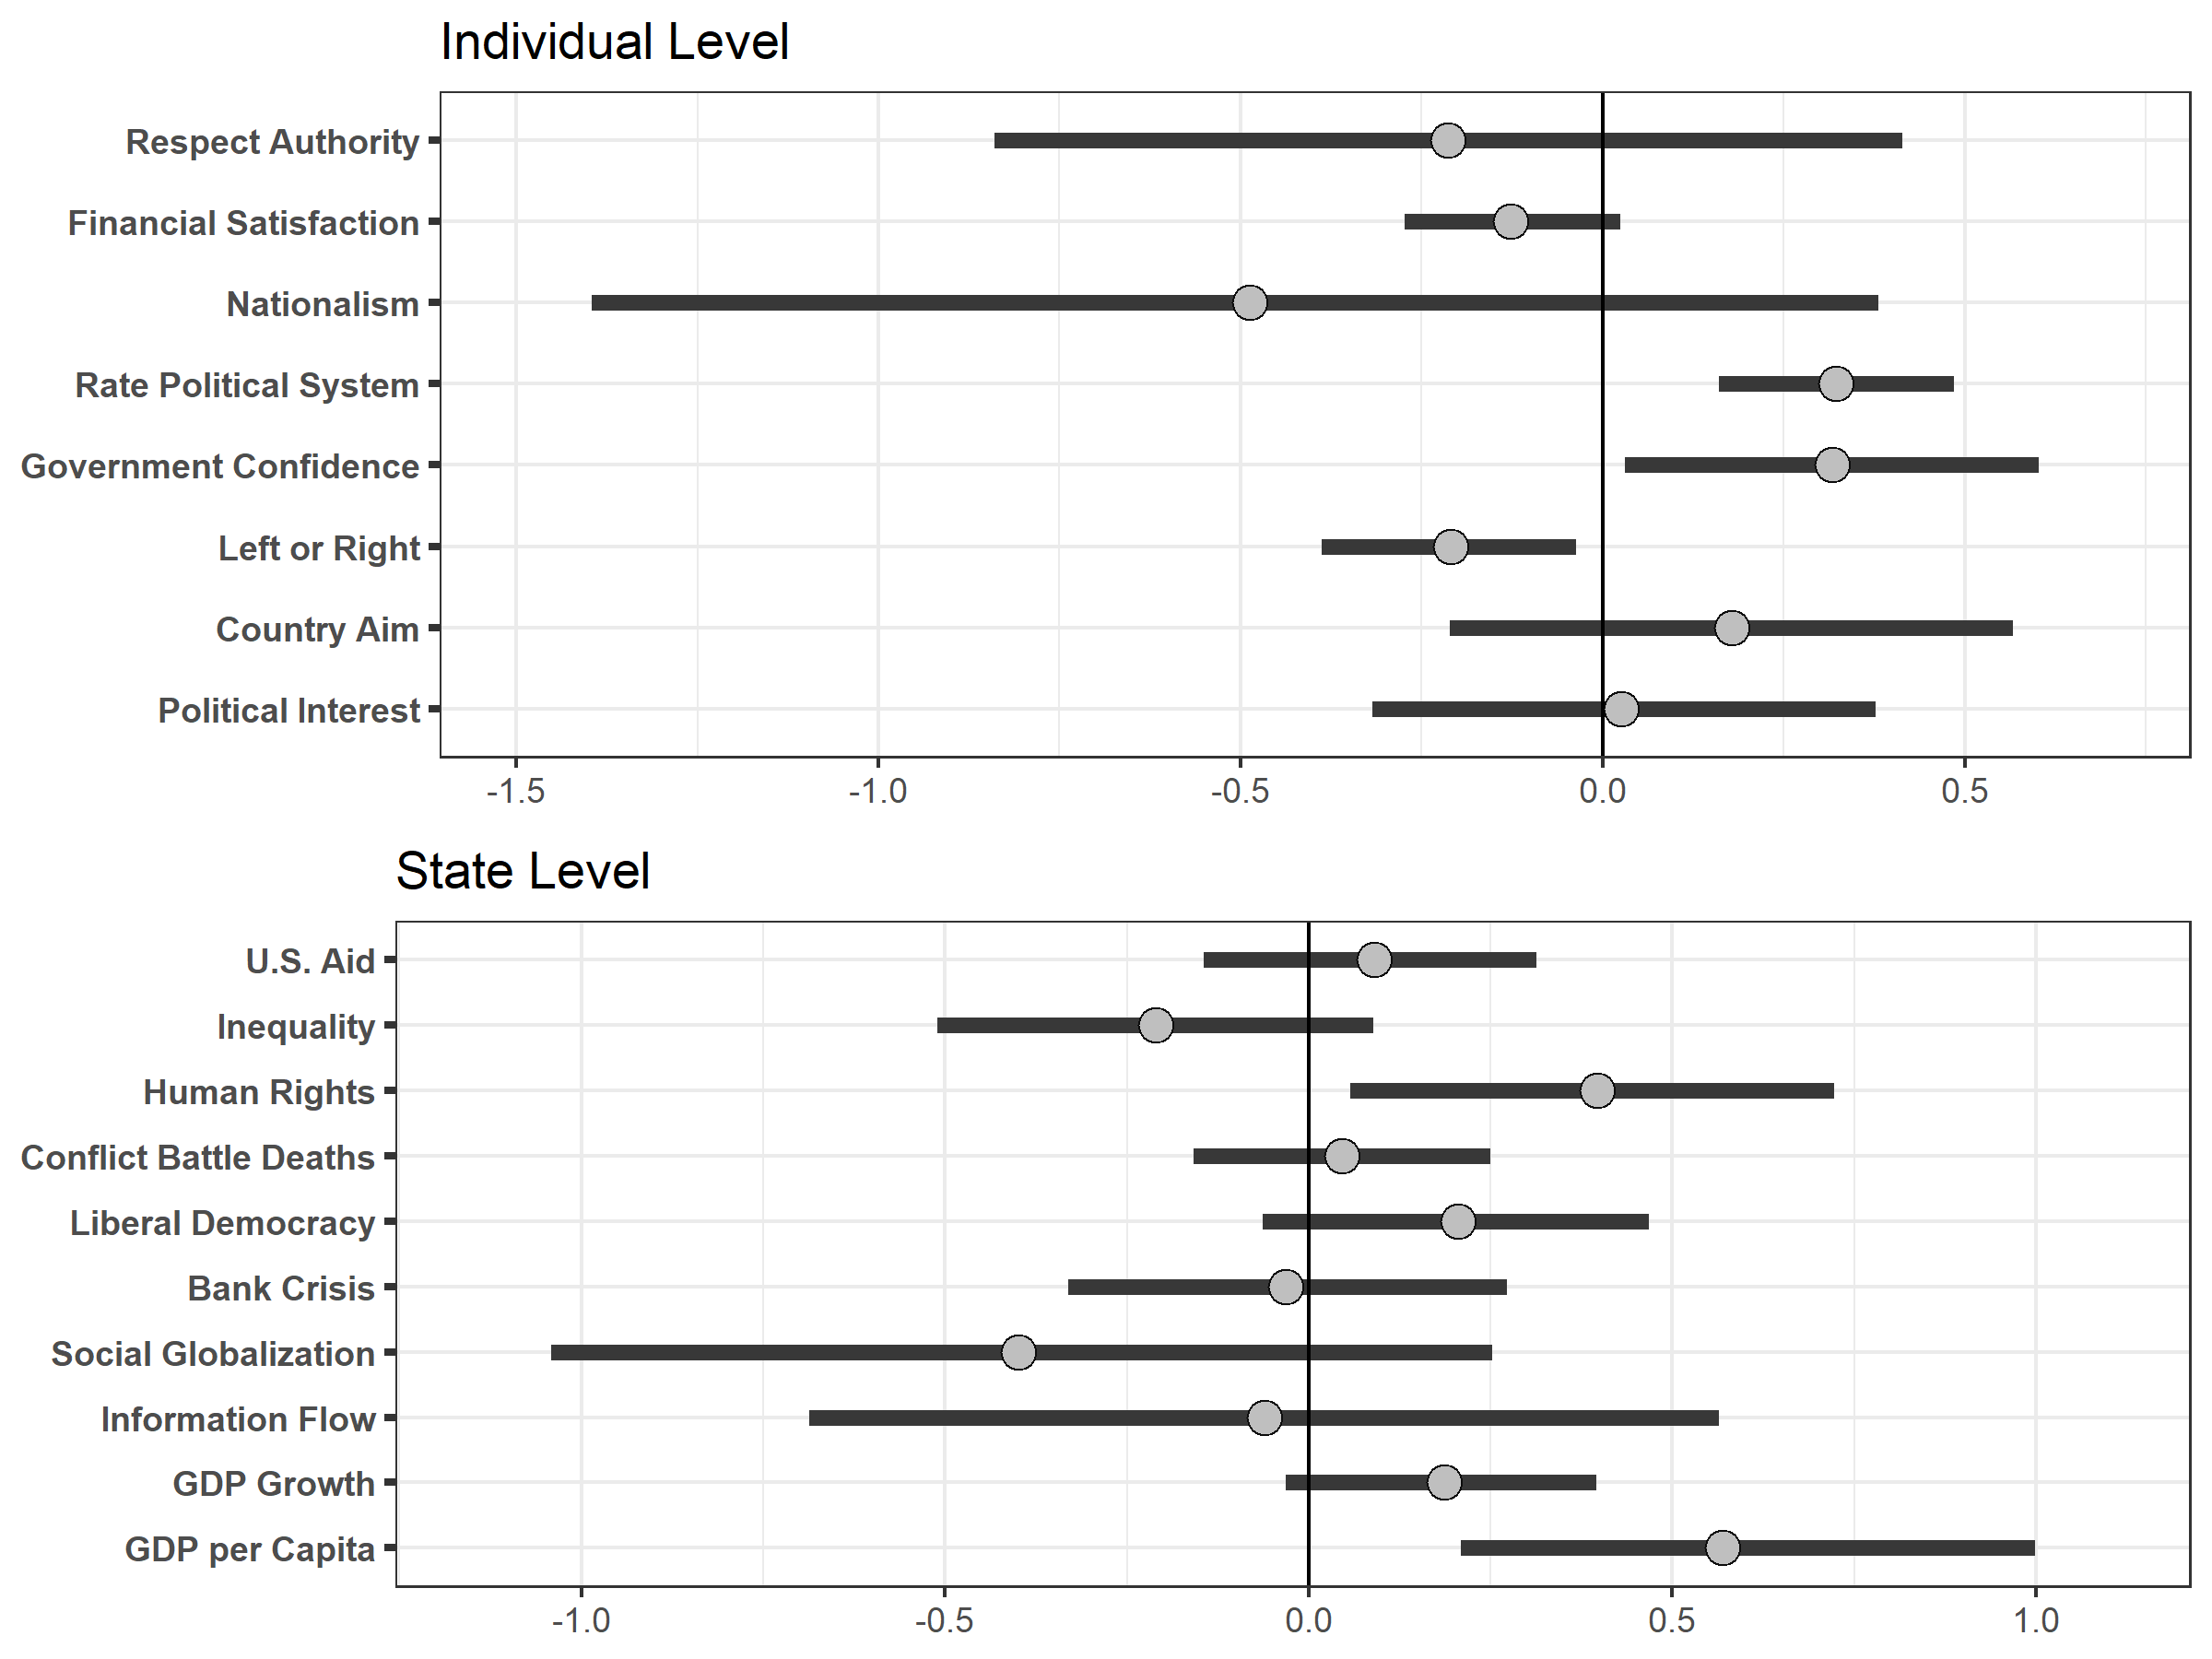
\includegraphics[width = .95\textwidth]{other-levels-vars.png}
\caption{Estimated association between individual and state level variables and the probability of high democratic support. Point estimates mark the posterior median, and error bars summarize the 90\% credible interval.}
\label{fig:other-levels-vars} 
\end{figure}


Some individual and state-level variables also impact support for democracy outside the United States. 
Because we average the individual variables at the country-year level to facilitate binomial model fitting, the individual coefficient estimates compare averages across observations.
Higher average ratings of the political system and confidence in the government in a country increase the likelihood of high democratic support. 
Countries where individuals are more right-wing on average express lower support for democracy. 
The nationalism and financial satisfaction averages are also negative, but are more uncertain.


At the state level, GDP per capita is positively associated with high democratic support. 
The GDP growth, human rights and liberal democracy coefficient estimates are largely positive, but consistent with slight negative relationships. 
The income inequality and social globalization coefficients are mostly negative with substantial uncertainty. 


\begin{figure}
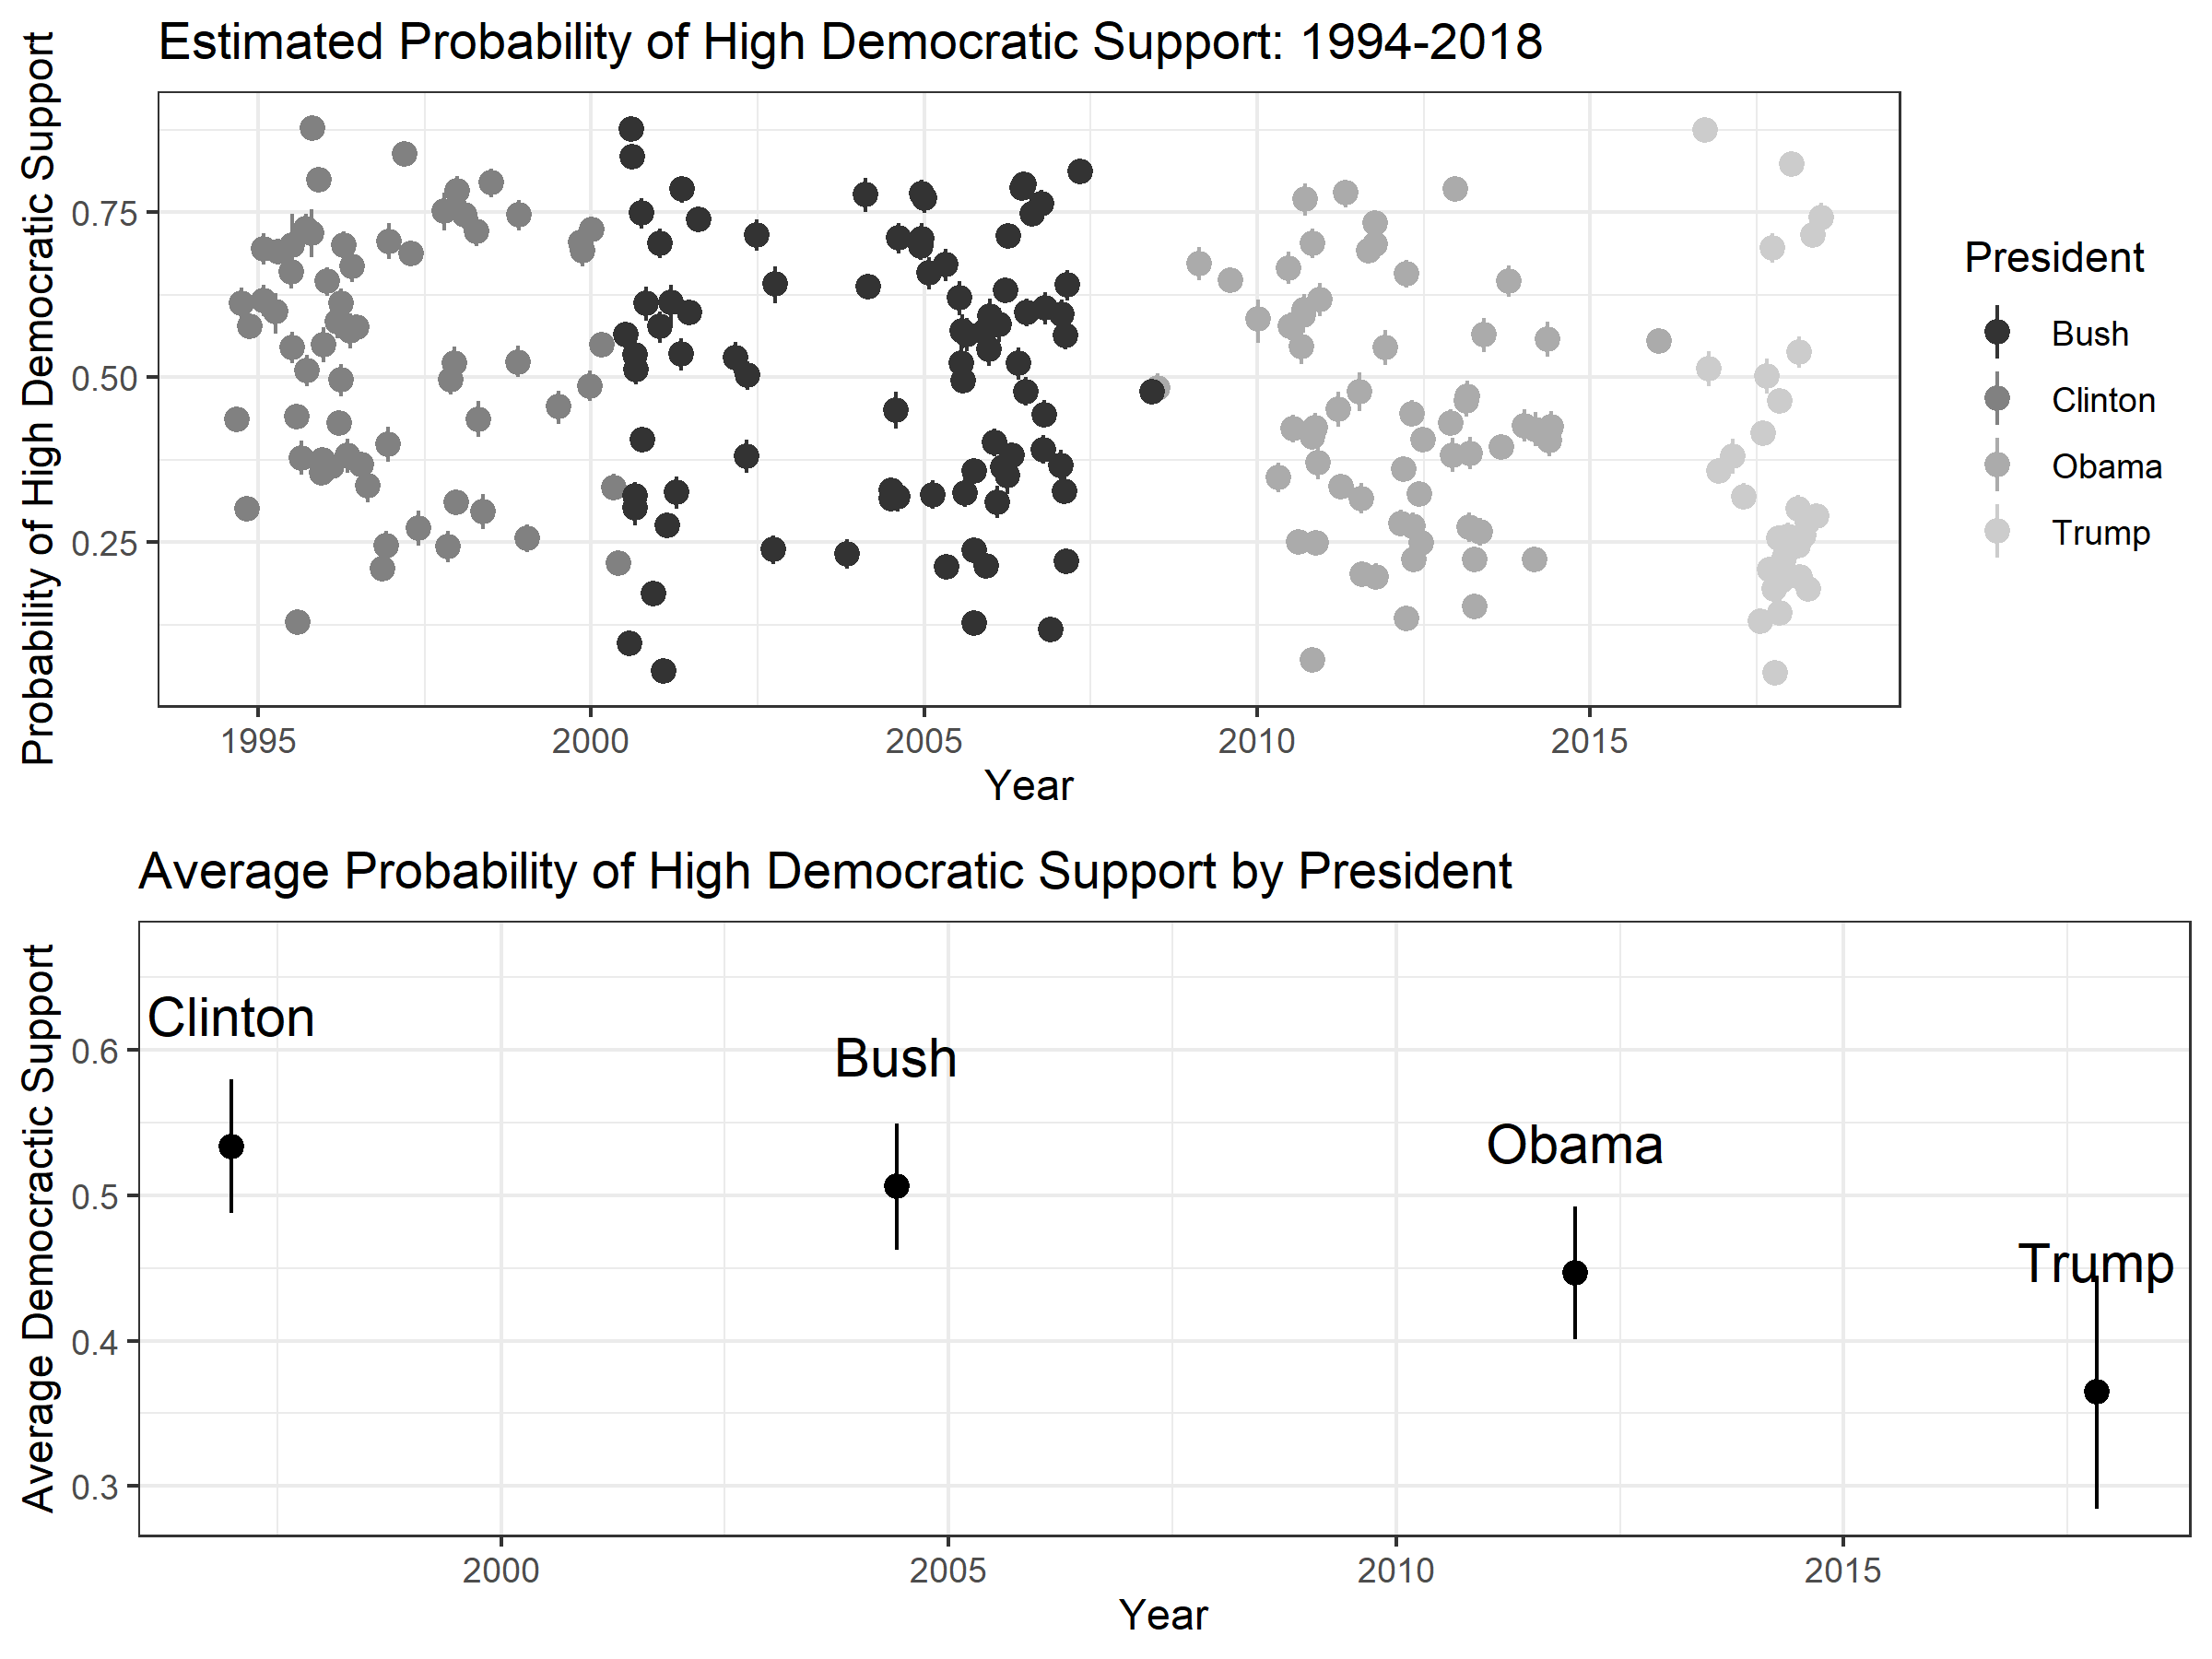
\includegraphics[width = .95\textwidth]{theta-est.png}
\caption{Estimated probability of high democratic support in country-year observations from 1994 to 2019, with averages by presidential administration. In the top panel, each point marks the estimated probability of high democratic support in a country-year observation, and the error bars summarize the 90\% credible interval. The bottom panel is the average of the posterior medians for each president. Estimates from before 1994 omitted to make the plot more legible.  }
\label{fig:theta-est} 
\end{figure}


\autoref{fig:theta-est} plots the estimated probability of high democratic support for each country-year observation in the WVS from 1994 to 2019. 
Each point is the estimated $\theta$ parameter in the binomial logit model.
This is the probability of a success ---high democratic support--- in the number of binomial trials given by the number of respondents. 


There are some notable patterns in democratic support over time.
The first is that the average of the $\theta$ parameters by President declines gradually over time, then drops dramatically during the Trump administration.  
The Trump average reflects a cluster of state-year observations with low probabilities of high democratic support. 
Interestingly, several estimates from the Trump administration are higher than any from the Obama administration, which might suggest global polarization in democratic support. 


\section{Trump and Democratic Support in Asia}

The models in the manuscript find a negative impact of the Trump administration on support for democracy in Asia. 
In this section of the appendix, we explore that finding further. 
To do so, we fit separate models to each state in Asia that had WVS data before and after Trump took office in early 2017. 


Fitting separate models for each state is a simple way to assess whether the impact of the Trump administration and other factors varies by country. 
It also allows us to draw on the full range of the democratic support variable, instead of simplifying it to a dummy, as in the manuscript. 
Because democratic support takes on relatively few integer values, we fit Bayesian ordinal logit models with flexible outcome thresholds using BRMS \citep{Buerkner2017}.
The lack of cross-sectional variation in these analyses meant we could only include two state and year level variables without introducing perfect multicollinearity into the model. 
We therefore included a national economic growth variable and the Trump administration dummy, in addition to a series of controls at the individual level. 
For each state, we fit models to five imputed datasets, and then combined them into a single posterior, following standard practice. 


We find that the Trump presidency reduced support for democracy throughout Asia. 
\autoref{fig:asia-state-trump} plots the estimated coefficient on the Trump administration dummy variable from each model of democratic support over time in Asian states. 
Most of the coefficient estimates are negative, and most are substantively large as well. 


\begin{figure}
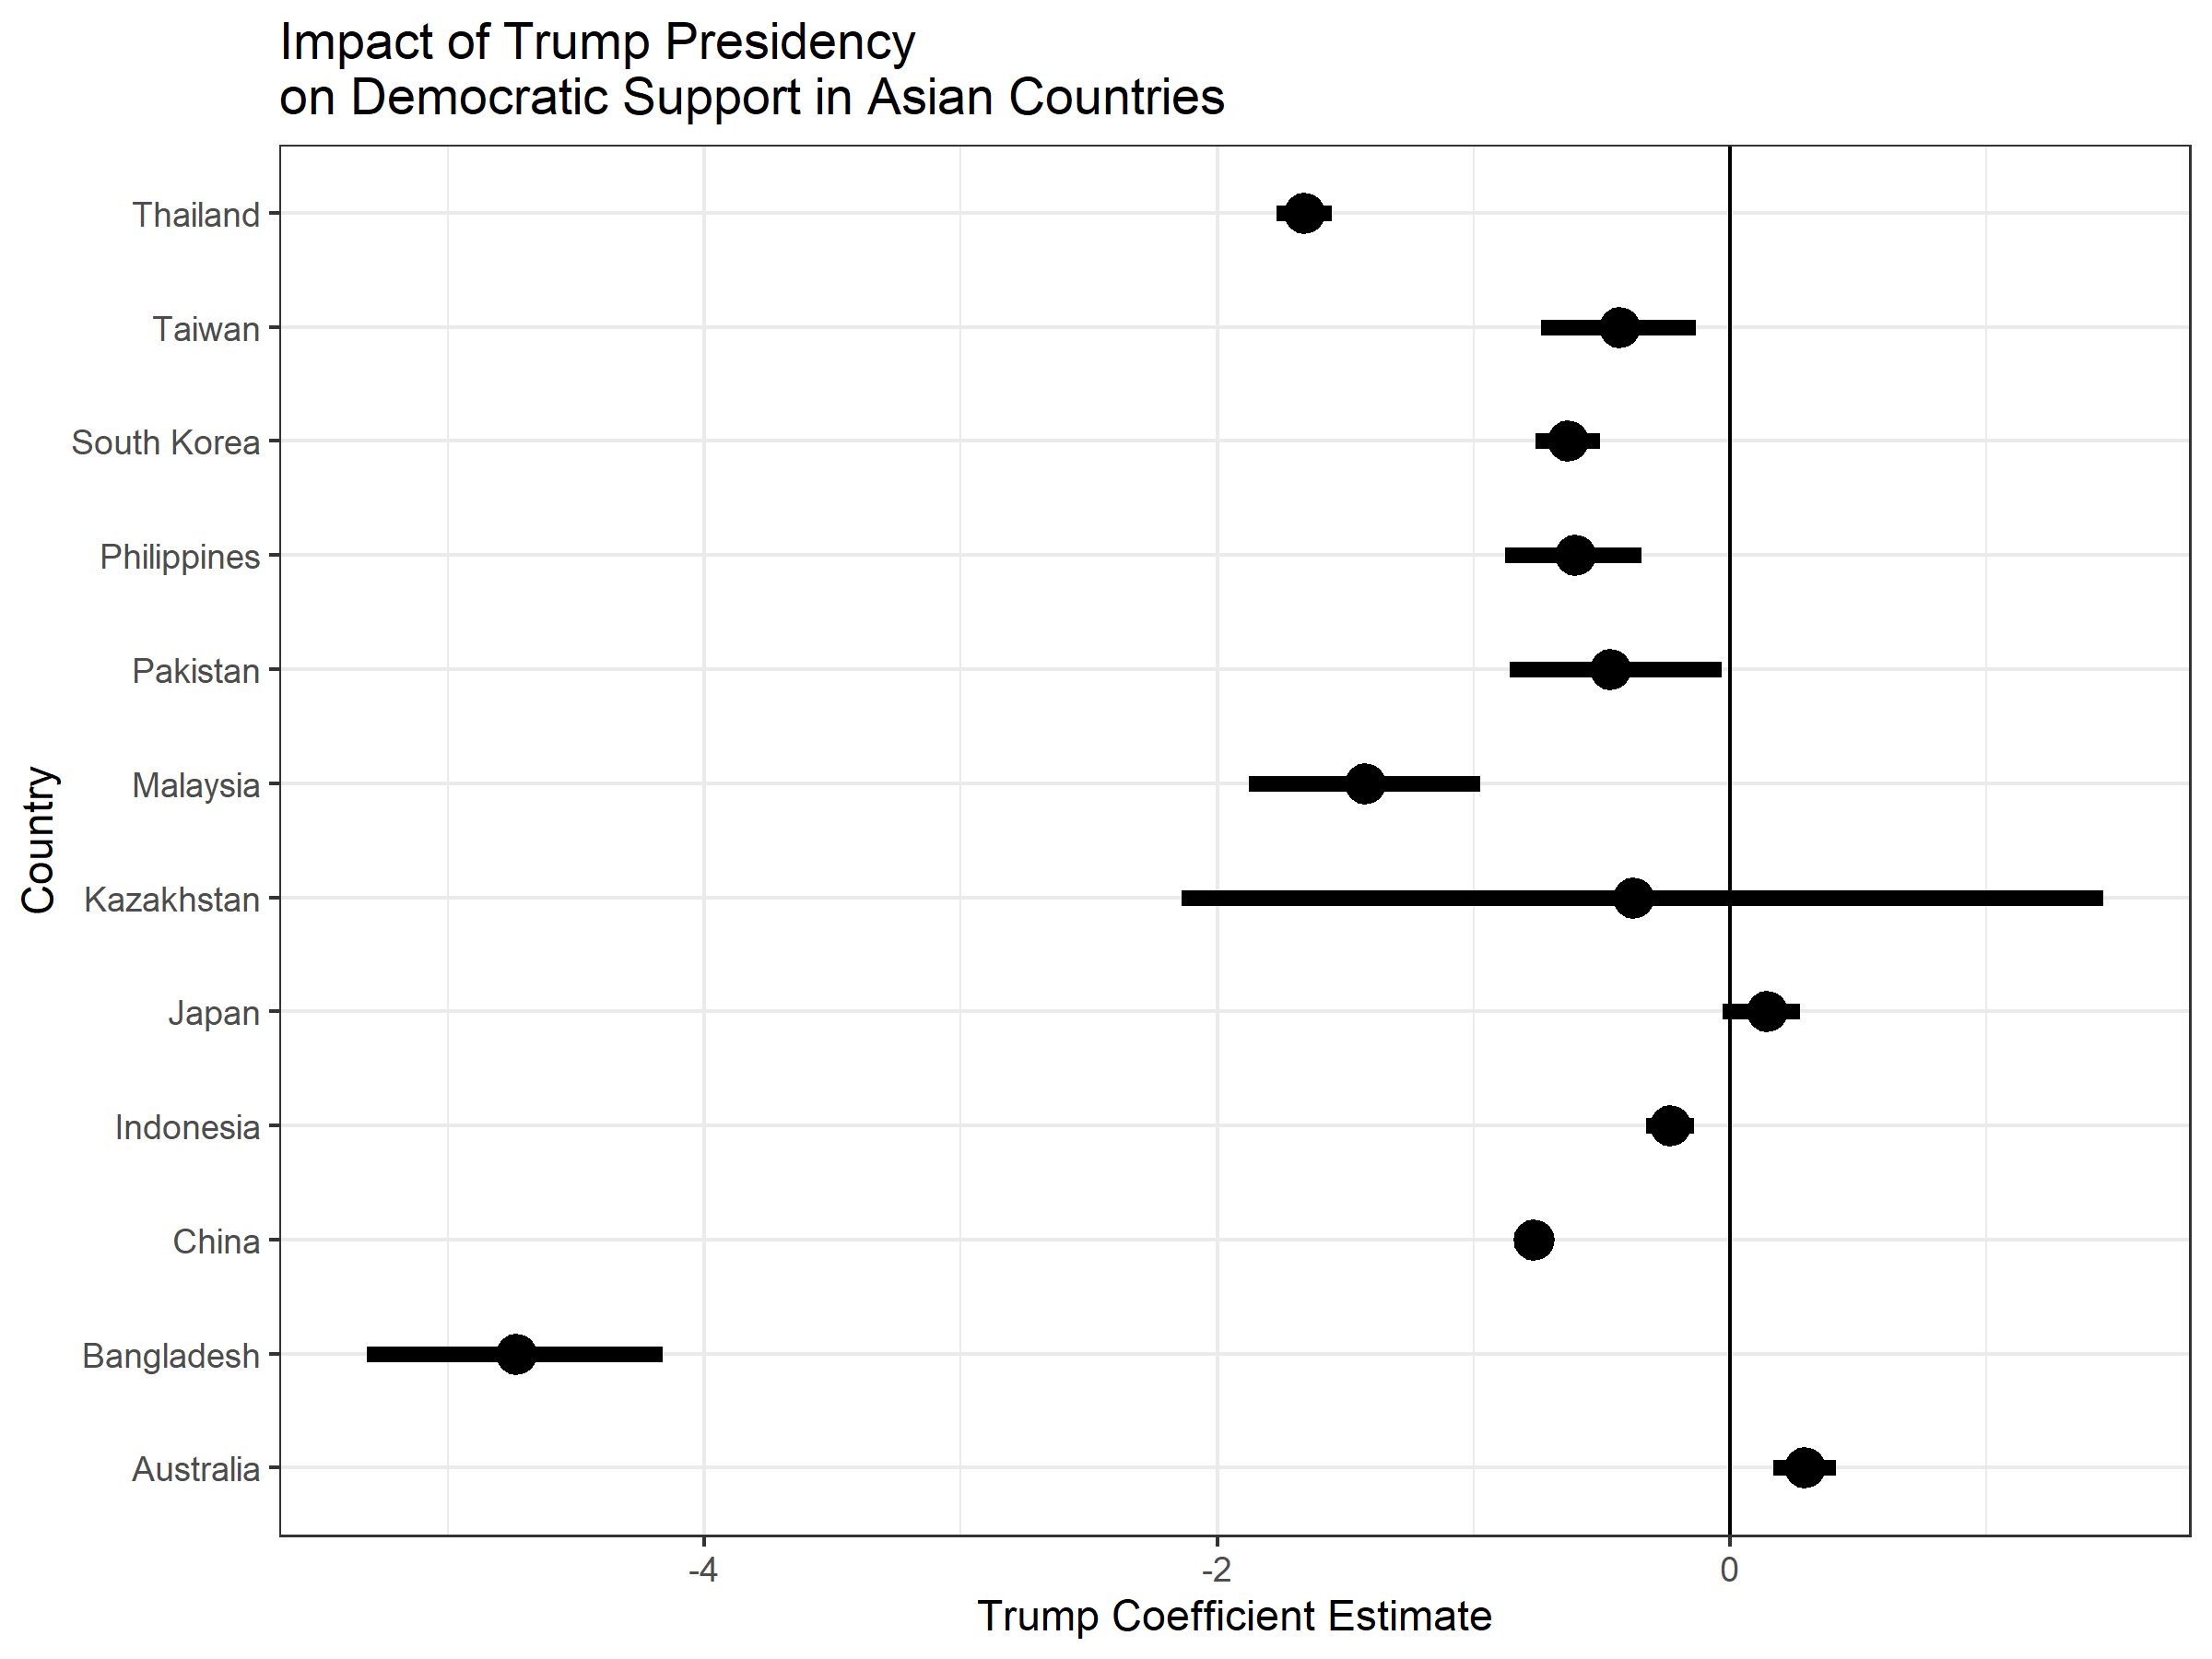
\includegraphics[width = .95\textwidth]{asia-state-trump.png}
\caption{Estimated association between Donald Trump's presidency and public support for democracy in Asian countries, 1980 to 2019. Point estimates mark the posterior median, and error bars summarize the 90\% credible interval. Coefficient estimates reflect pooled estimates from five Bayesian ordered logit models fit to five imputed datasets for each state.}
\label{fig:asia-state-trump} 
\end{figure}


The Trump effect is largest in Bangladesh, but this may reflect that only three WVS waves covered Bangladesh, which creates limited temporal variation in that model. 
The Kazakhstan coefficient has substantial uncertainty for similar reasons. 
Only in Australia is the Trump administration correlated with increased democratic support. 


Indonesia, Thailand, Taiwan, the Philippines, South Korea, Pakistan, Malaysia and China all saw lower public support for democracy during the Trump administration. 
The common change in a group with such varied characteristics gives some credence to a common trend or shock. 
The mechanism likely differs across these countries, however. 
South Korea and the Philippines are U.S. treaty allies and Taiwan has close ties to the United States. 
China's relationship with the Trump administration was often antagonistic. 
Pakistan has some ties to the U.S., along with close relations with China. 


\newpage


\section{WVS Coverage by Region and Presidency}


It is also possible that we estimate a negative relationship between Trump and democratic support in Asia but not in other regions due to better data coverage in that region. 
The WVS proceeds country by country, and our sample lacks data on key variables in 2020, so we lose out on data from later in the seventh wave.\footnote{With completely missing data for most countries, imputation has less value.}
Thus, as \autoref{fig:theta-reg} shows, we have more estimates for countries in Asia and consistent coverage of the Americas, with more sparse coverage in Africa and Europe. 



\begin{figure}
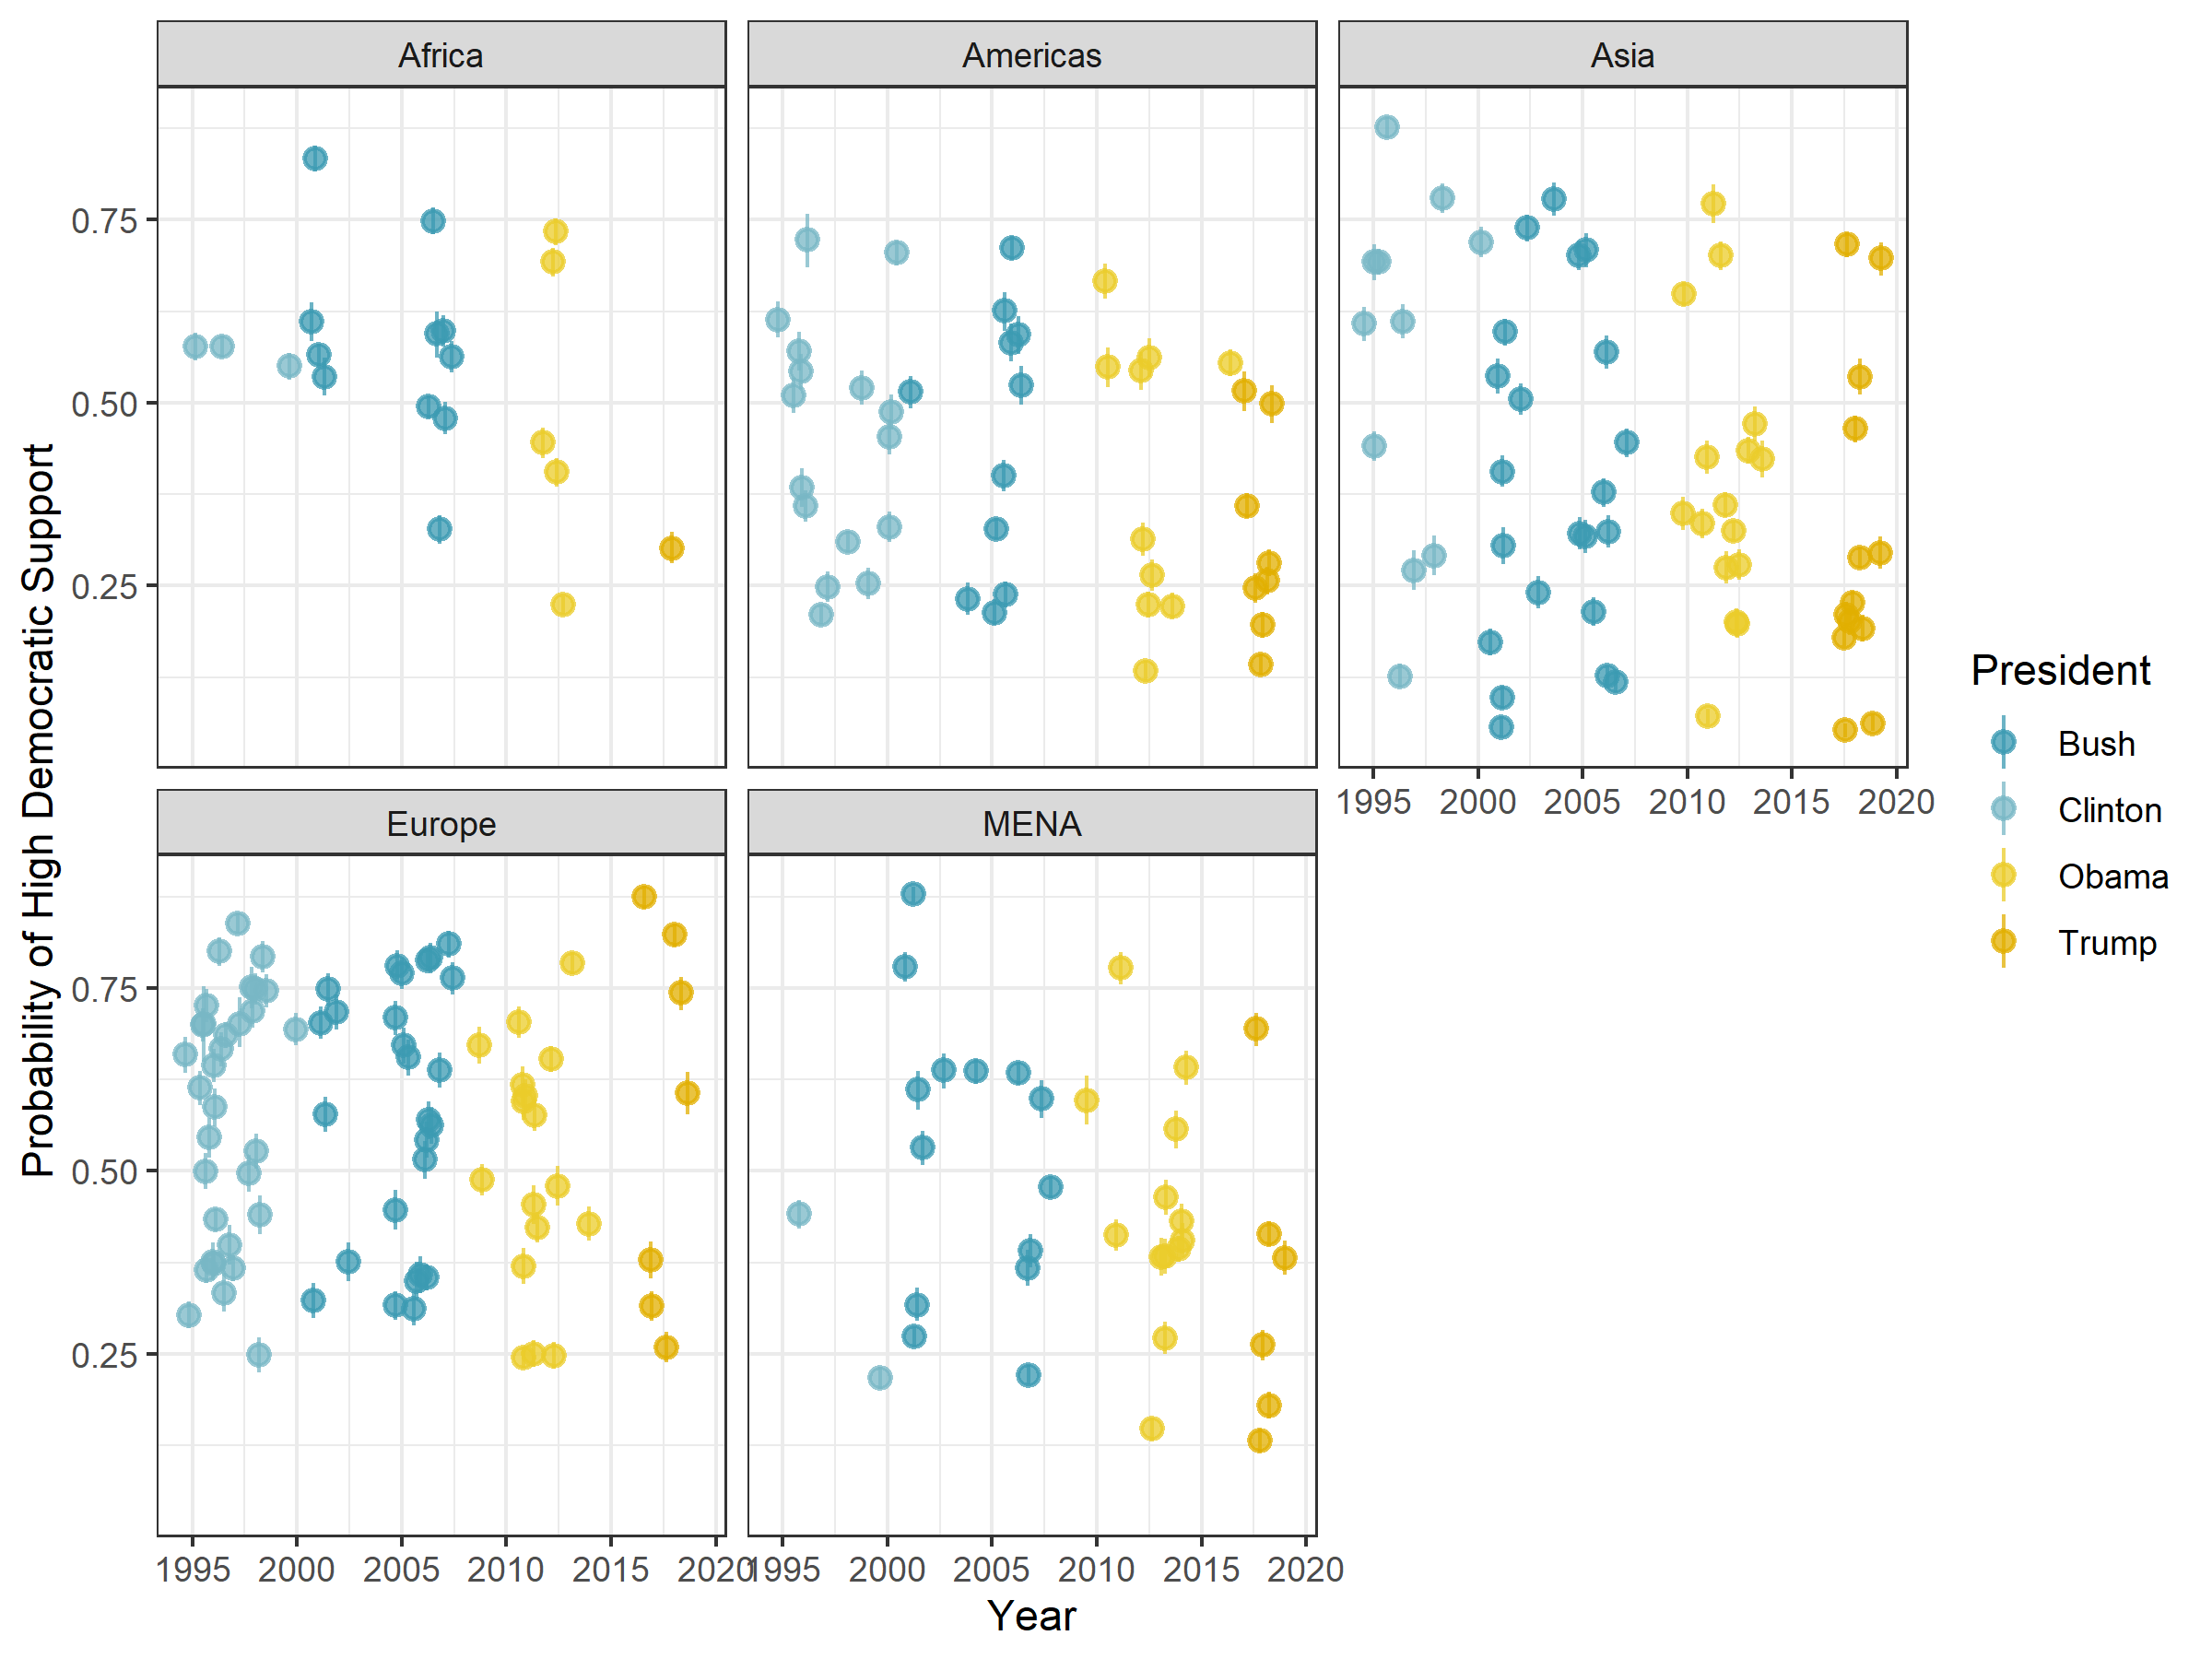
\includegraphics[width = .95\textwidth]{theta-reg.png}
\caption{Estimated probability of high democratic support by region from multilevel model with regional varying slopes. Colors differentiate between presidential administrations. MENA stands for Middle East and North Africa.}
\label{fig:theta-reg} 
\end{figure}


The Trump finding may carry over into other regions, but data coverage limits our ability to assess this. 
A similar relationship is plausible in Africa and the Middle East. 
Although the Trump presidency is negatively associated with democratic support in the Americas, the association is weaker than in Asia. 


The likely patterns in Europe are less clear. 
On the one hand, the Australian and Japanese estimates from the analysis of Asian countries suggests that the Trump administration was less likely to damage perceptions of democracy among wealthy consolidated democracies.
On the other, democratic support fell in South Korea and Taiwan during the Trump administration.
Thus, Trump may have done little damage to democratic support in Europe, or reduced support in countries he frequently interacted with. 


\autoref{fig:theta-reg} further indicates that the largely negative association between the Clinton administration and support for democracy in the Middle East and North Africa is likely the result of sparse data. 
There are only two countries with WVS data during the Clinton administration. 
Larger samples from the region during other presidencies show substantial variation in support for democracy that drives up average democratic support. 


%\section{Democracy and the Trump Effect} 
%
%
%As the analysis of Asia countries suggests, consolidated democracies and other states respond differently to international examples. 
%To further explore this, we modified the varying slopes model and instead of dividing states by region, divided them by democratic status. 
%Using data on the mean and standard deviation of the VDEM liberal democracy measure, we created three groups of states. 


  
 
\bibliography{../../MasterBibliography} 




\end{document}
